\begin{center}
\textbf{实验三:数据库应用系统的开发}
\end{center}

\section{实验目的}
初步掌握数据库应用系统分析设计的基本方法;进一步提高分析与解决问题
的综合能力;初步掌握数据库建模工具的使用方法;熟悉掌握 CS 或 BS 结构的
数据库应用系统开发的整个过程。

\section{实验预备内容}
\begin{enumerate}
  \item 阅读教材《数据库系统概论》设计与应用开发篇。
  \item 阅读实验使用的数据库管理系统的相关帮助文档。
  \item 学习数据库建模工具的使用;
  \item 学习某种应用编程开发工具及其连接访问数据库的方法;
  \item 学习设计、开发数据库应用系统的相关知识.
\end{enumerate}

\section{实验环境}
\begin{itemize}
  \item OS: Linux;
  \item DBMS: OpenGauss;
  \item Programming language: Python, JavaScript;
  \item Others: Vim
\end{itemize}

\section{实验内容}

背景自定义,使用某种应用开发编程工具(Java、Python、PHP、VC 等)结
合华为云平台数据库 openGauss 完成一个数据库应用系统(BS、CS 模式均可)
的分析、设计与实现。

基本要求:能实现对数据库中数据的插入、删除、修改、查询、统计查询等
功能,做到界面友好、使用方便。掌握程序访问数据库中数据的技术方法,进一
步提高分析与解决问题的综合能力。

实验三如果系统工作量较大可 2-3 人团队合作完成,但要选定组长负责并
明确任务分工,保障每人的工作量饱满。

\subsection{系统选题需求情况及任务分工情况说明}
(团队合作需细化说明每个队员负责的具体功能模块,工作量占比)

\begin{itemize}
  \item 选题: 笔记管理系统;
  \item 分工: 单人负责前端和后端, 工作量占比 100\%.
\end{itemize}

\subsection{系统的概念数据模型设计}
(E-R图)

笔记管理系统中包含两类实体, 即``用户''和``笔记'', ``用户''和``笔记''实体之间的关系属于一对多的关系.

\begin{figure}[H]
  \begin{center}
    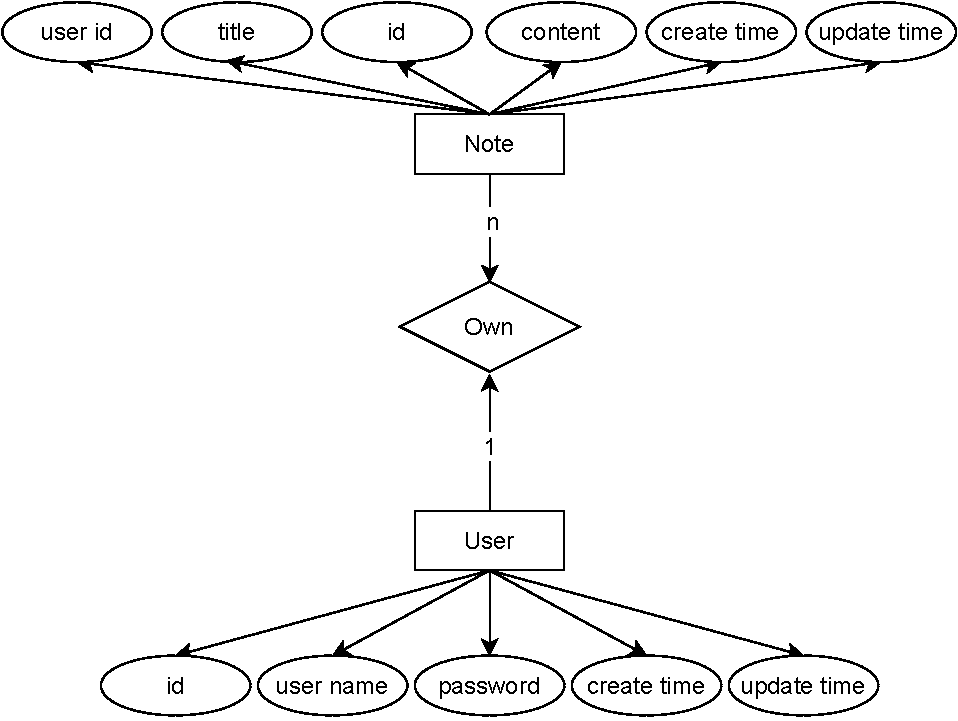
\includegraphics[page=1,scale=0.45]{./resources/er.pdf}
  \end{center}
  \caption{Entity Relationship Graph}
\end{figure}

\subsection{系统中每张表的说明}
\begin{table}[H]
  \caption{用户}
  \begin{center}
    \begin{tabular}[c]{ll}
      \hline
      列 & 说明 \\
      \hline
      id & 唯一的用户 ID \\
      username & 用户名 \\
      password & 加密后的密码 \\
      create\_time & 用户创建时间 \\
      update\_time & 用户信息更新时间 \\
      \hline
    \end{tabular}
  \end{center}
\end{table}

\begin{table}[H]
  \caption{笔记}
  \begin{center}
    \begin{tabular}[c]{ll}
      \hline
      列 & 说明 \\
      \hline
      id & 唯一的笔记 ID \\
      title & 笔记的标题 \\
      content & 笔记的详细内容 \\
      create\_time & 笔记的创建时间 \\
      update\_time & 笔记的更新时间 \\
      user\_id & 笔记的拥有者, 外键, 参照用户表 \\
      \hline
    \end{tabular}
  \end{center}
\end{table}

\subsection{系统运行环境配置}
(安装操作说明,前端与后台数据库连接用到的关键语句说明)

\begin{itemize}
  \item OS: Linux;
  \item DBMS: OpenGauss;
  \item Programming language: Python;
  \item Python 3rd-party package: Django, psycopg2;
  \item PostgreSQL library: libpq-dev;
  \item 前端与后台数据库连接用到的关键语句说明: Django 针对不同的 DBMS
    使用不同的引擎, 但使用相同的数据模型, 提升了应用程序与 DBMS 的独立性.
\end{itemize}

\subsection{系统主要功能界面介绍}
(需使用截图)

\begin{figure}[H]
  \begin{center}
    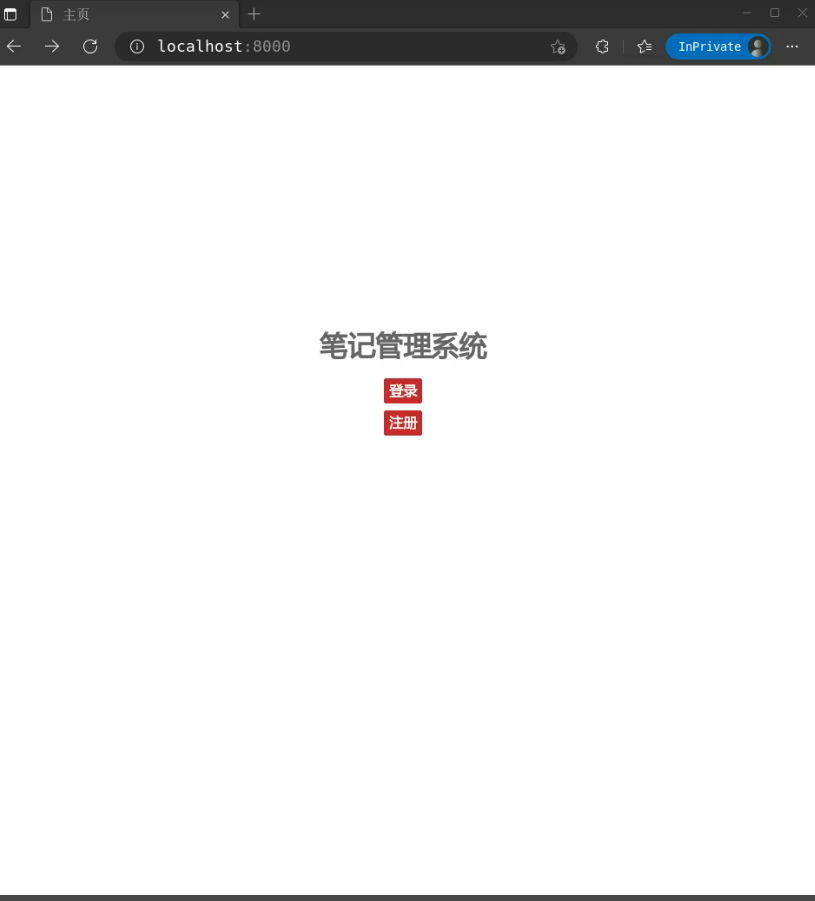
\includegraphics[width=0.95\textwidth]{./figures/home_page.png}
  \end{center}
  \caption{主页}
\end{figure}

\begin{figure}[H]
  \begin{center}
    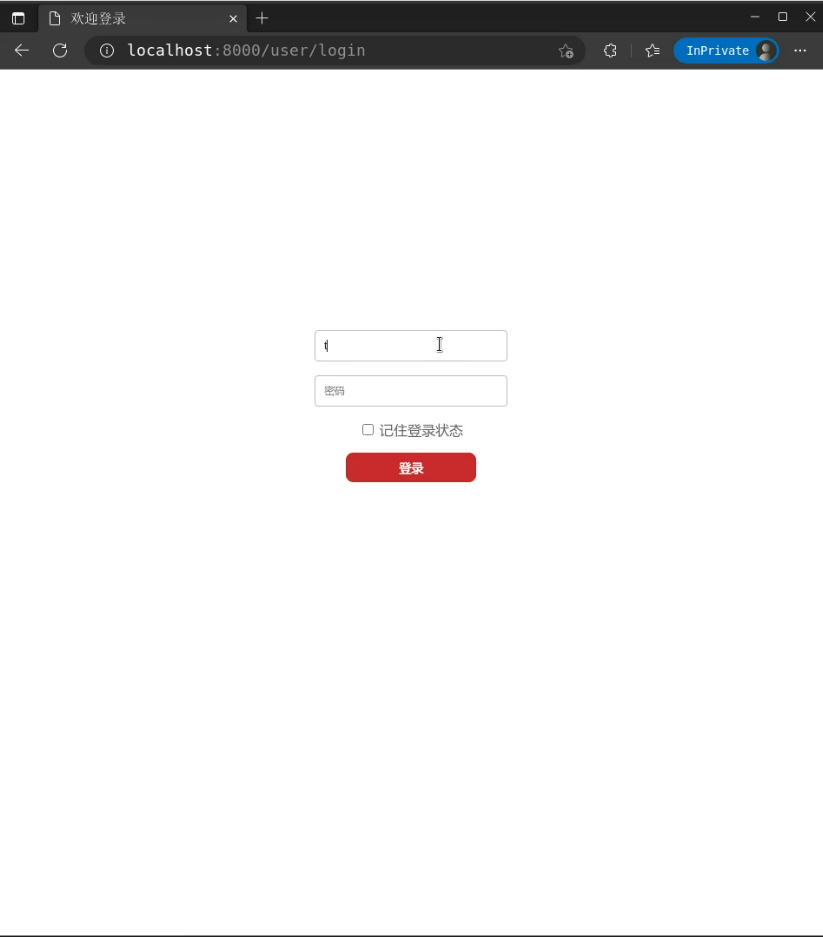
\includegraphics[width=0.95\textwidth]{./figures/login_page.png}
  \end{center}
  \caption{登录页}
\end{figure}

\begin{figure}[H]
  \begin{center}
    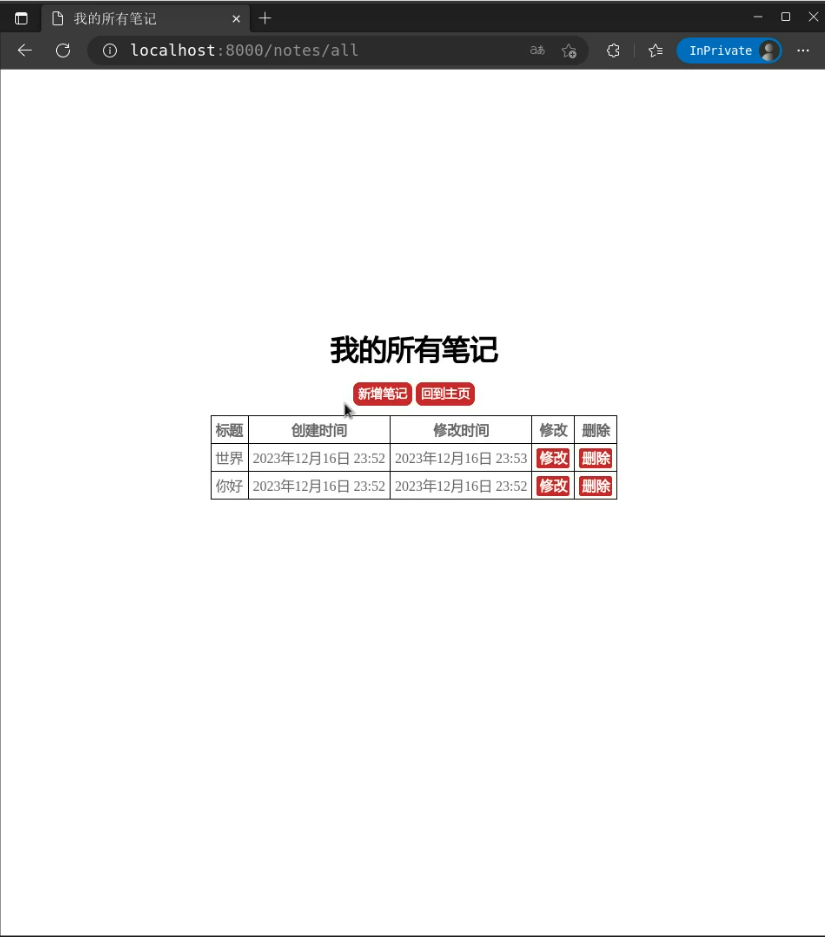
\includegraphics[width=0.95\textwidth]{./figures/list_note_page.png}
  \end{center}
  \caption{笔记列表页}
\end{figure}

\begin{figure}[H]
  \begin{center}
    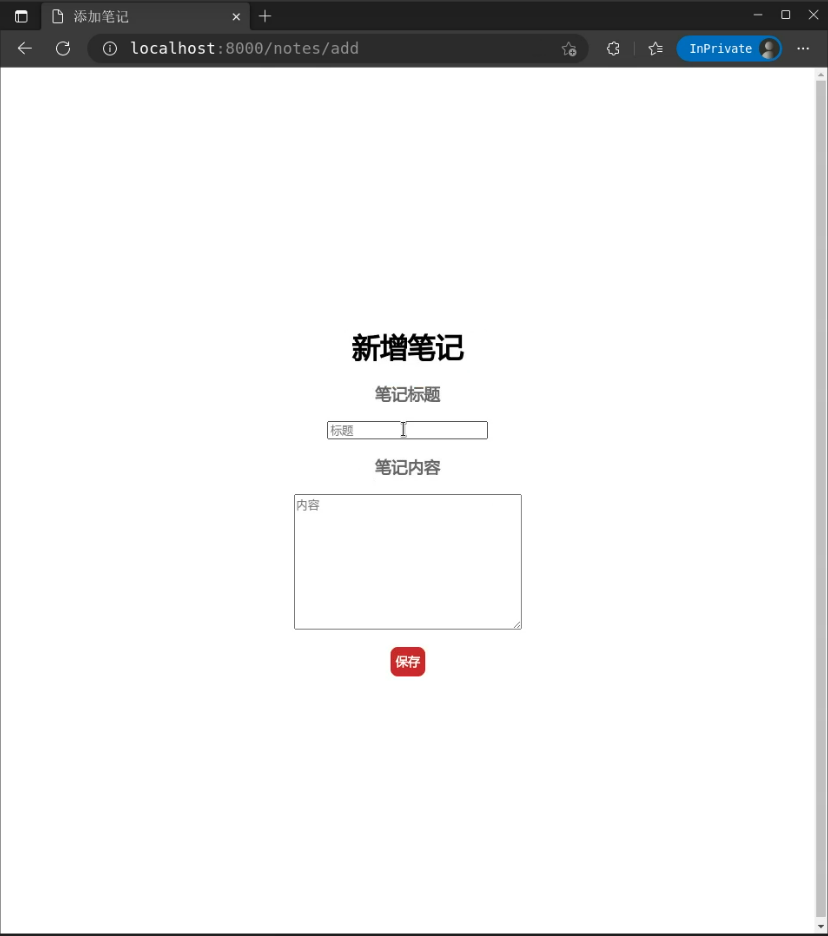
\includegraphics[width=0.95\textwidth]{./figures/add_note_page.png}
  \end{center}
  \caption{新建笔记页}
\end{figure}

\begin{figure}[H]
  \begin{center}
    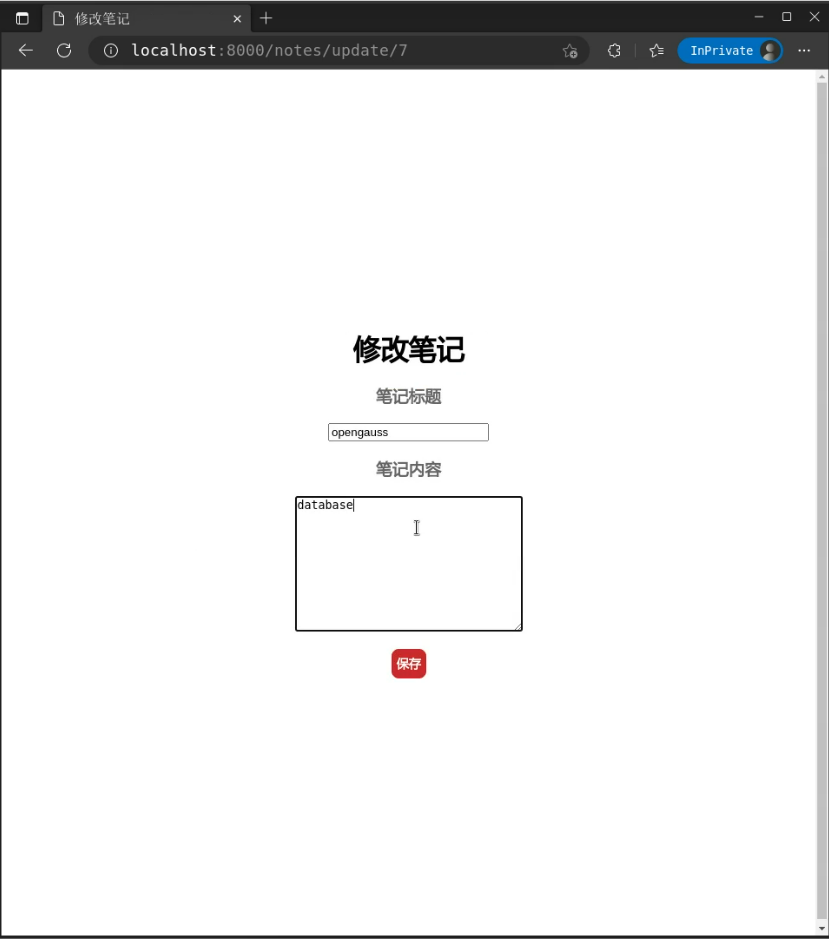
\includegraphics[width=0.95\textwidth]{./figures/update_note_page.png}
  \end{center}
  \caption{更新笔记页}
\end{figure}

\section{实验结果总结}
(分析系统运行效果,说明系统优缺点及改进方向)

\begin{itemize}
  \item 系统运行效果: 总体上实现了对数据库的增删改查的功能;
  \item 优点: 适用于多用户的笔记管理, 笔记的增删改查简单、高效;
  \item 缺点: 页面元素过少, 页面不够美观;
  \item 改进方向:
    \begin{enumerate}
      \item 改善 UI;
      \item 提高系统的健壮性;
      \item 增加对 Markdown 语法的支持;
      \item 增加对数学公式的支持;
      \item 增加对图片内容的支持;
      \item 增加对 SQL 注入的防范;
      \item 增加对 CSRF 的防范.
    \end{enumerate}
\end{itemize}

\section{编程工作总结}
(系统开发所付出的努力、面临的困难,自学了哪些相关知识;
自己负责什么模块,遇到什么问题怎么解决的,有没有自己创新的设计,
开发的体会与收获等。请认真完成,不少于 500 字。
注意:分组完成的同学只说明自己完成的工作,不要写别人的工作)

说明:团队合作的同学,组长的报告需写完整,组员报告实验内容一至五项可以标
注为``见组长报告'',组员和组长都需在报告封面上组长的姓名后括号标注组长。

\subsection{系统开发所付出的努力}
在开发此系统的过程中, 我付出了很大的努力, 包括解决所面临的诸多困难,
自学开发系统所需的相关知识,
负责前端和后端的开发以及代码的调试、环境的部署等模块, 并在遇到问题时请教
同学、搜寻相关资料和博客、查阅官方的相关文档, 成功地解决问题.

\subsection{面临的困难}
由于此系统是我一个人开发的, 这意味着我需要同时学习前端和后端的知识,
同时因为 OpenGauss 数据库管理系统是基于 PostgreSQL 的, 而 PostgreSQL 和
MySQL 存在着差异, 从 MySQL 过渡到 PostgreSQL 也是需要成本的.

\subsection{自学的知识}
开发中主要用到了前端、后端以及数据库管理系统的使用的相关知识, 包括:
\begin{itemize}
  \item HTML, CSS, JavaScript;
  \item Python, Django;
  \item OpenGauss 的安装和使用.
\end{itemize}

\subsection{负责模块}
此系统是由我一个人完成的, 其中包含:
\begin{itemize}
  \item 系统运行环境的配置和部署;
  \item 系统开发环境的配置和部署;
  \item 数据库的概念模型设计;
  \item 数据库的模式设计;
  \item 数据库的建立与维护;
  \item 前端界面的开发;
  \item 后端接口的开发;
  \item 前后端数据交换接口的定义;
  \item 前后端的联调.
\end{itemize}

\subsection{遇到的问题及其解决}
Django 无法成功连接到 OpenGauss 数据库管理系统:
修改 OpenGauss 的配置文件, 使其同时支持 MD5 和 SHA 加密通信,
修改 OpenGauss 绑定的地址和端口, 最后重启 OpenGauss
数据库管理系统即可解决此问题.

\subsection{开发的体会和收获}
在此次开发过程中, 我分别学习了前端和后端的相关知识, 了解了前后端分离的
设计范式, 对数据库理论在实际数据库系统中的应用有了深刻的理解,
进一步了解数据库的模式设计对数据库系统高效、稳定地运行的重要性,
体会到 SQL 的强大和不足之处, 认识了 MVC 模式的核心思想, 即:
功能的解耦和功能的模块化,
认识到数据在信息时代的重要性, 对开发中存在的一些安全问题有了初步的理解.
